\documentclass[aspectratio=169]{beamer} % dvipsnames gives more built-in colors
\usepackage{graphicx} % Required for inserting images
\usepackage{transparent}
\usepackage{float}
\usepackage{tikz}
\usepackage{amsmath}
\usepackage[font=scriptsize,labelfont=bf]{caption}
\usepackage{algorithmicx}
\usepackage{listings}
\usepackage{animate}
\renewcommand{\footnotesize}{\tiny}

\usepackage{tikz}
\usepackage{tikz-cd}
\tikzcdset{scale cd/.style={every label/.append style={scale=#1},
    cells={nodes={scale=#1}}}}

\usepackage{babel}  
\usepackage{siunitx}  
\sisetup{locale = DE}
\usepackage{multicol}
\usepackage{listings}

\usetikzlibrary{arrows.meta, angles, quotes, calc}

%\usepackage[sorting=none]{biblatex}
\usepackage[german=guillemets]{csquotes}
\setquotestyle{english}
%\addbibresource{bibliography.bib}

\usetheme{ufr}
\usecolortheme{ufr}

\newcommand{\bC}{\mathbb{C}}
\newcommand{\bD}{\mathbb{D}}

\title{What you needa know about Yoneda}
\author{Emma Bach (she/her)}
\date{Seminar on Functional Programming and Logic, Summer Semester 2025}

\begin{document}

{
\usebackgroundtemplate{
        \transparent{0.1}    
        \hspace{7cm}
        
\includegraphics[width=0.7\paperwidth]{logos/ufr-siegel-grey.png}
        }

\begin{frame}[plain]
    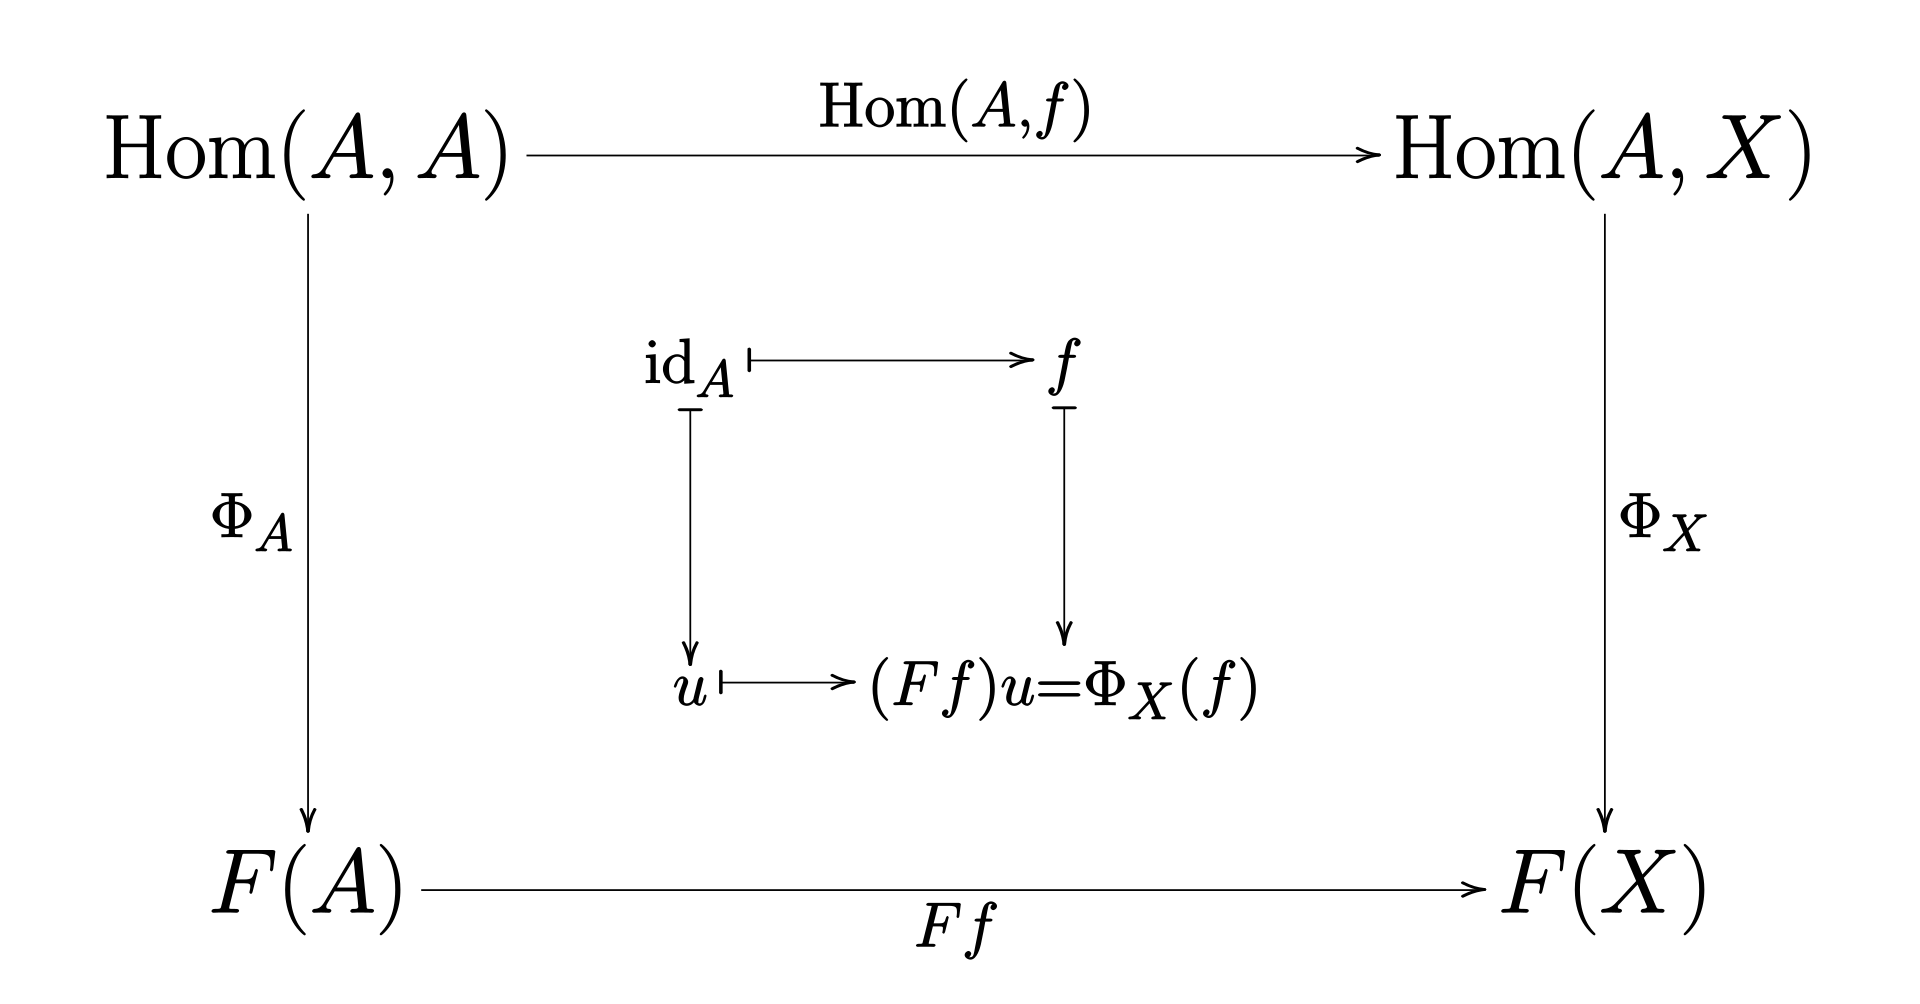
\includegraphics[width=0.4\paperwidth]{figures/Yoneda_lemma_cd.svg.png}
    \titlepage
\end{frame}

\begin{frame}{Motivation}
 \begin{itemize}
  \item A common sentiment in many cultures is the idea that people are defined by how they interact with their surroundings.
  \pause\item ``\textit{Tell me your company, and I will tell you what you are.}''\footnote{Quoted as a proverb in \textit{Don Quixote}}
  \pause\item The Yoneda Lemma is the result of applying this way of thinking to mathematical objects within the extremely general setting of \textit{category theory}.
  \pause\item Far-reaching consequences throughout abstract algebra, set theory, and functional programming.
 \end{itemize}
\end{frame}

\begin{frame}[fragile]{Categories}
\begin{columns}
\column{0.3\textwidth}
% https://q.uiver.app/#q=WzAsNCxbMCwwLCJBIl0sWzIsMCwiQiJdLFsyLDIsIkMiXSxbNywyXSxbMCwxLCJmIl0sWzEsMiwiZyJdLFswLDIsImYgXFxjaXJjIGciLDJdLFswLDAsImlkXzEiXSxbMSwxLCJpZF8yIl0sWzIsMiwiaWRfMyIsMix7InJhZGl1cyI6LTN9XV0=
\[\begin{tikzcd}
	A && B \\
	\\
	&& C &&&&& {}
	\arrow["{id_1}", from=1-1, to=1-1, loop, in=55, out=125, distance=10mm]
	\arrow["f", from=1-1, to=1-3]
	\arrow["{f \circ g}"', from=1-1, to=3-3]
	\arrow["{id_2}", from=1-3, to=1-3, loop, in=55, out=125, distance=10mm]
	\arrow["g", from=1-3, to=3-3]
	\arrow["{id_3}"', from=3-3, to=3-3, loop, in=305, out=235, distance=10mm]
\end{tikzcd}\]
\column{0.7\textwidth}
A \textit{category} $\bC$ consists of:
\begin{itemize}
 \pause\item a collection $|\bC|$ of \textit{objects};
 \pause\item for all $A, B \in |\bC|$, a collection $\bC(A, B)$ of \textit{morphisms} from $A$ to $B$;
 \pause\item for all $A \in |\bC|$, an \textit{identity morphism} $id_A \in \bC(A, A)$;
 \pause\item an associative \textit{composition morphism} $f \circ g \in \bC(A,C)$ for each pair of morphisms $f \in \bC(A,B)$, $g \in \bC(A,B)$.
\end{itemize}
If $\bC(A, B)$ is a set, we call it the \textit{homset} from $A$ to $B$.
\end{columns}
\end{frame}
\begin{frame}[fragile]{Examples}
\begin{columns}
\column{0.3\textwidth}
\[\begin{tikzcd}
	A && B \\
	\\
	&& C &&&&& {}
	\arrow["{id_A}", from=1-1, to=1-1, loop, in=55, out=125, distance=10mm]
	\arrow["{f}", from=1-1, to=1-3]
	\arrow["{f \circ g}"', from=1-1, to=3-3]
	\arrow["{id_B}", from=1-3, to=1-3, loop, in=55, out=125, distance=10mm]
	\arrow["{g}", from=1-3, to=3-3]
	\arrow["{id_C}"', from=3-3, to=3-3, loop, in=305, out=235, distance=10mm]
\end{tikzcd}\]
\column{0.7\textwidth}
The Category $\mathbb{S}et$
\begin{itemize}
 \pause\item Objects are sets
 \pause\item A morphism $f \in \bC(A,B)$ is a function $A \to B$
 \pause\item The most important category for this talk (and arguably in general)
\end{itemize}
\end{columns}
\end{frame}
\begin{frame}[fragile]{Examples}
\begin{columns}
\column{0.3\textwidth}
% https://q.uiver.app/#q=WzAsNCxbMCwwLCIxIl0sWzIsMCwiMiJdLFsyLDIsIjMiXSxbNywyXSxbMCwxLCJmIDogMSBcXGxlcSAyIl0sWzEsMiwiZyA6IDIgXFxsZXEgMyJdLFswLDIsImYgXFxjaXJjIGcgOiAxIFxcbGVxIDMiLDJdLFswLDAsImlkXzEgOiAxIFxcbGVxIDEiXSxbMSwxLCJpZF8yIDogMiBcXGxlcSAyIl0sWzIsMiwiaWRfMyA6IDMgXFxsZXEgMyIsMix7InJhZGl1cyI6LTN9XV0=
\[\begin{tikzcd}
	1 && 2 \\
	\\
	&& 3 &&&&& {}
	\arrow["{id_1 : 1 \leq 1}", from=1-1, to=1-1, loop, in=55, out=125, distance=10mm]
	\arrow["{f : 1 \leq 2}", from=1-1, to=1-3]
	\arrow["{f \circ g : 1 \leq 3}"', from=1-1, to=3-3]
	\arrow["{id_2 : 2 \leq 2}", from=1-3, to=1-3, loop, in=55, out=125, distance=10mm]
	\arrow["{g : 2 \leq 3}", from=1-3, to=3-3]
	\arrow["{id_3 : 3 \leq 3}"', from=3-3, to=3-3, loop, in=305, out=235, distance=10mm]
\end{tikzcd}\]
\column{0.7\textwidth}
Order Categories
\begin{itemize}
 \pause\item Let $S$ be a set with a partial ordering $\leq$
 \pause\item Objects are the elements of $S$
 \pause\item A morphism $f \in \bC(A,B)$ represents the fact $A \leq B$
\end{itemize}
\end{columns}
\end{frame}
%
%
%
\begin{frame}[fragile]{Haskell Functors}
\begin{itemize}
 \item In Haskell, a \textit{functor} is defined as an instance of the following typeclass:
 \pause\begin{verbatim}
  class Functor f where
    fmap :: (a -> b) -> f a -> f b
 \end{verbatim}
 \pause Where the following \textit{functor laws} are assumed to hold:
  \pause \begin{verbatim}
  fmap id = id
  fmap f (fmap g x) == fmap (f . g) x
 \end{verbatim}
\end{itemize}
\end{frame}
%
%
%
\begin{frame}[fragile]{Functors in Category Theory}
\begin{columns}
\column{0.3\textwidth}
% https://q.uiver.app/#q=WzAsNCxbMCwwLCJBIl0sWzAsMiwiRihBKSJdLFsyLDAsIkIiXSxbMiwyLCJGKEIpIl0sWzAsMSwiRiIsMCx7InN0eWxlIjp7ImJvZHkiOnsibmFtZSI6ImRhc2hlZCJ9fX1dLFswLDIsImYiLDJdLFsyLDMsIkYiLDIseyJzdHlsZSI6eyJib2R5Ijp7Im5hbWUiOiJkYXNoZWQifX19XSxbMSwzLCJGKGYpIl1d
\[\begin{tikzcd}
	A && B \\
	\\
	{F(A)} && {F(B)}
	\arrow["f"', from=1-1, to=1-3]
	\arrow["{F(f)}", from=3-1, to=3-3]
\end{tikzcd}\]
\column{0.7\textwidth}
\begin{itemize}
 \item General Functors are almost identical to Haskell Functors.
 \pause\item In general, a functor is a map $F : \bC \to \bD$.
 \begin{itemize}
  \pause\item An object $A \in |\bC|$ is mapped to an object $F(A) \in |\bD|$
  \pause\item A morphism $f \in \bC(A,B)$ is mapped to a morphism $F(f) \in \bD(F(A), F(B))$
 \end{itemize}
 \pause\item Functors are structure preserving.
 \begin{itemize}
  \pause\item $F(id_A) = id_{F(A)}$
  \pause\item $F(f \circ g) = F(f) \circ F(g)$
 \end{itemize}
\end{itemize}
\end{columns}
\end{frame}
\iffalse
\begin{frame}[fragile]{Functors in Programming}
 \begin{verbatim}
     data Maybe a = Nothing | Just a
 \end{verbatim}
 \begin{itemize}
  \item \texttt{Maybe} defines a functor $\texttt{Maybe} : \mathbb{S}et \to \mathbb{S}et$
  \item A set \texttt{a} is mapped to a set \texttt{Maybe a}
  \item Given a function $f : a \to b$, we can define a function $\texttt{Maybe}\ f : \texttt{Maybe}\ a \to \texttt{Maybe}\ b$  as follows:
  \begin{align*}
   \texttt{Maybe}\ f(a) = \begin{cases}
                           \texttt{Nothing} & \texttt{Maybe}\ a  = \texttt{Nothing}\\
                           \texttt{Just}\ f(a) & \texttt{Maybe}\ a  = \texttt{Just}\ a\\
                          \end{cases}
  \end{align*}
  \item In Haskell notation:
  \begin{verbatim}
    fmap :: (a -> b) -> Maybe a -> Maybe b
    fmap _ Nothing = Nothing
    fmap f (Just x) = Just (f x)
  \end{verbatim}

 \end{itemize}
\end{frame}
\fi
\begin{frame}[fragile]{Homfunctors}
\begin{columns}
\column{0.3\textwidth}
 % https://q.uiver.app/#q=WzAsMyxbMCwwLCJBIl0sWzIsMiwiQyJdLFsyLDAsIkIiXSxbMCwxLCJmIFxcY2lyYyBnIiwxXSxbMCwyLCJmIiwxXSxbMiwxLCJnIiwxXV0=
\[\begin{tikzcd}
	A && B \\
	\\
	&& C
	\arrow["f"{description}, from=1-1, to=1-3]
	\arrow["{f \circ g}"{description}, from=1-1, to=3-3]
	\arrow["g"{description}, from=1-3, to=3-3]
\end{tikzcd}\]
% https://q.uiver.app/#q=WzAsNCxbNCwwXSxbMCwwLCJcXHtpZF9BXFx9Il0sWzIsMCwiXFx7ZlxcfSJdLFsyLDIsIlxce2YgXFxjaXJjIGdcXH0iXSxbMSwyLCJmIFxcY2lyYyIsMV0sWzIsMywiZyBcXGNpcmMiLDFdLFsxLDMsImYgXFxjaXJjIGcgXFxjaXJjIiwxXV0=
\[\begin{tikzcd}
	{\{id_A\}} && {\{f\}} && {} \\
	\\
	&& {\{f \circ g\}}
	\arrow["{f \circ}"{description}, from=1-1, to=1-3]
	\arrow["{f \circ g \circ}"{description}, from=1-1, to=3-3]
	\arrow["{g \circ}"{description}, from=1-3, to=3-3]
\end{tikzcd}\]
\column{0.7\textwidth}
 \begin{itemize}
  \item For any category $\bC$, a homset $\bC(A,B)$ is a set of morphisms.
  \item We define a functor $\bC(A, -) : \bC \to \mathbb{S}et$:
  \begin{itemize}
    \item $\bC(A, -)$ maps an Object $B$ to the Homset $\bC(A,B)$
    \item A morphism $f : \bC(B,C)$ is mapped to the morphism $f \circ : \bC(A,B) \to \bC(A,C)$
  \end{itemize}
 \end{itemize}
 \end{columns}
\end{frame}
\begin{frame}{Natural Transformations}
\end{frame}
\begin{frame}{The Yoneda Embedding}
\end{frame}
\begin{frame}{The Yoneda Lemma}
Definition
\end{frame}
\begin{frame}{The Yoneda Lemma}
Proof
\end{frame}
\begin{frame}
 $\hdots$
\end{frame}
\begin{frame}{Instances of the Yoneda Lemma}
\begin{itemize}
 \item Cayley's theorem in group theory
 \item Countless theorems in algebra, particulary in algebraic topology
 \item Proofs by indirect inequality: $b \preceq a$ iff. $\forall c : (a \preceq c) \implies (b \preceq c)$
 \item Profunctor optics in functional programming
\end{itemize}

\end{frame}
\begin{frame}{Profunctor Optics}
\end{frame}

}

\end{document}
